\documentclass[a4paper]{article}

\usepackage{hyperref}

\newcommand{\triposcourse}{Markov Chains}
\newcommand{\triposterm}{Michaelmas 2020}
\newcommand{\triposlecturer}{Dr. R. Bauerschmidt}
\newcommand{\tripospart}{IB}

\usepackage{amsmath}
\usepackage{amssymb}
\usepackage{amsthm}
\usepackage{mathrsfs}

\usepackage{tikz-cd}

\usepackage{tikz}
\usetikzlibrary{automata,positioning}

\theoremstyle{plain}
\newtheorem{theorem}{Theorem}[section]
\newtheorem{lemma}[theorem]{Lemma}
\newtheorem{proposition}[theorem]{Proposition}
\newtheorem{corollary}[theorem]{Corollary}
\newtheorem{problem}[theorem]{Problem}
\newtheorem*{claim}{Claim}

\theoremstyle{definition}
\newtheorem{definition}{Definition}[section]
\newtheorem{conjecture}{Conjecture}[section]
\newtheorem{example}{Example}[section]

\theoremstyle{remark}
\newtheorem*{remark}{Remark}
\newtheorem*{note}{Note}

\title{\triposcourse{}
\thanks{Based on the lectures under the same name taught by \triposlecturer{} in \triposterm{}.}}
\author{Zhiyuan Bai}
\date{Compiled on \today}

\setcounter{section}{-1}

\begin{document}
    \maketitle
    This document serves as a set of revision materials for the Cambridge Mathematical Tripos Part \tripospart{} course \textit{\triposcourse{}} in \triposterm{}.
    However, despite its primary focus, readers should note that it is NOT a verbatim recall of the lectures, since the author might have made further amendments in the content.
    Therefore, there should always be provisions for errors and typos while this material is being used.
    \tableofcontents
    \section{Introduction}
A Markov chain consists of a state space and a set of probabilities of going from a state to another.
We can either draw the transition as a directed graph with probability labels, or we can write out the transition matrix, with the $i,j$ entry taken to be the probability of going from state $i$ to state $j$.
For example, we can take the state space as $\{1,2,3\}$ with transition rules drawn as the following graph:
\begin{center}
    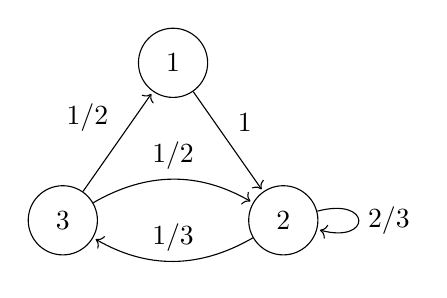
\begin{tikzpicture}
        \node[state] at (0,2) (1){$1$};
        \node[state] at (1.4,0) (2){$2$};
        \node[state] at (-1.4,0) (3){$3$};

        \draw[every loop]
        (1) edge[auto=left] node {$1$} (2)
        (3) edge[auto=left] node {$1/2$} (1)
        (2) edge[loop right] node {$2/3$} (2)
        (3) edge[bend left, auto=left] node {$1/2$} (2)
        (2) edge[bend left, auto=right] node {$1/3$} (3);
    \end{tikzpicture}
\end{center}
It then has transition matrix
$$\begin{pmatrix}
    &1&\\
    &2/3&1/3\\
    1/2&1/2&
\end{pmatrix}$$
Obvious we want the sum of each row to be $1$ as you have to transit somewhere (including your current location) from where you were.\\
We can have a more involved example.
Consider the state space $\{0,\ldots,6\}$ with transition rules
\begin{center}
    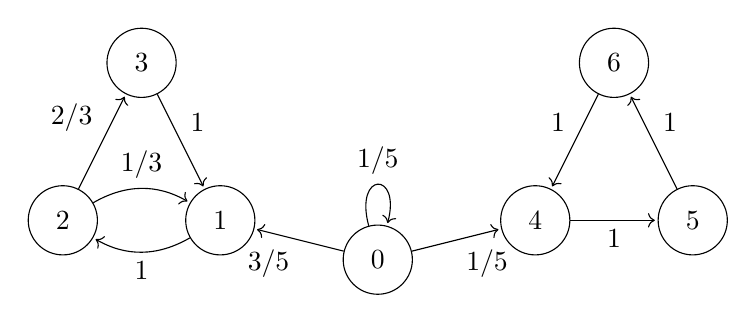
\begin{tikzpicture}
        \node[state] at (0,-0.5) (0){$0$};
        \node[state] at (-2,0) (1){$1$};
        \node[state] at (-4,0) (2){$2$};
        \node[state] at (-3,2) (3){$3$};
        \node[state] at (2,0) (4){$4$};
        \node[state] at (4,0) (5){$5$};
        \node[state] at (3,2) (6){$6$};

        \draw[every loop]
        (0) edge[auto=right] node {$1/5$} (4)
        (4) edge[auto=right] node {$1$} (5)
        (5) edge[auto=right] node {$1$} (6)
        (6) edge[auto=right] node {$1$} (4)
        (0) edge[auto=left] node {$3/5$} (1)
        (1) edge[bend left, auto=left] node {$1$} (2)
        (2) edge[bend left, auto=left] node {$1/3$} (1)
        (2) edge[auto=left] node {$2/3$} (3)
        (3) edge[auto=left] node {$1$} (1)
        (0) edge[loop above] node {$1/5$} (0);
    \end{tikzpicture}
\end{center}
There are many questions we can ask about a Markov chain.
For example, what is the probability of hitting one node from another eventually?
In the example above, some are obvious:
The probability of hitting $6$ eventually from $0$ is $1/5+(1/5)^2+\cdots=1/4$, and the probability of hitting $3$ eventually from $0$ is actually $1$.\\
We can ask other questions.
For example, what is the average number of steps to get from $1$ to $3$?
This turns out to be $3$.
Also, what is the long-run proportion of time to spend on $2$ if one starts at $1$?
It is $3/8$ as one can verify.\\
Throughout this course, we will attempt to come up with systematic ways to compute these things for a given Markov chain.\\
Another thing to observe is that in this specific example, we can group the states into three groups: $\{0\},\{1,2,3\}$ and $\{4,5,6\}$.
One can see that we cannot leave a group and go back with positive probability.
We call these communicating classes of a Markov chain.
    \section{Definitions and Basic Properties}
We will make the following standing assumptions:
First, the state space $I$ is a countable set which we will almost always label as $\{1,2,\ldots\}$.
Also, we will be working in a probability space $(\Omega,\mathscr F,\mathbb P)$ where all relevant random variables are defined.
\begin{definition}
    A sequence of random variables $(X_n)_{n=0,1,\ldots}$ is a Markov chain if, for all $n\ge 0$ and $i_0,\ldots,i_{n+1}\in I$,
    $$\mathbb P[X_{n+1}=i_{n+1}|X_0=i_0,\ldots,X_n=i_n]=\mathbb P[X_{n+1}=i_{n+1}|X_n=i_n]$$
    given that these conditional probabilities are well-defined.\\
    A Markov chain is homogeneous if for all $i,j\in I$,
    $$\mathbb P[X_{n+1}=j|X_n=i]=\mathbb P[X_1=j|X_0=i]$$
\end{definition}
We are only interested in homogeneous Markov chains, so afterwards when we mention a Markov chain, we always mean a homogeneous one.\\
Then, a Markov chain is characterised by the initial distribution $\lambda=(\lambda_i)_{i\in I}$ given by $\lambda_i=\mathbb P[X_0=i]$ and the transition matrix $P=(p_{ij})_{i,j\in I}$ with $p_{ij}=\mathbb P[X_1=j|X_0=i]$.\\
Note that $\lambda$ is a distribution as $\lambda_i$ is always nonnegative and sums up to $1$.
$P$, at the same time, is a stochastic matrix, i.e. $p_{ij}$ is a distribution for every $i\in I$.
\begin{definition}
    $(X_n)$ is a Markov chain with initial distribution $\lambda$ and transition matrix $P$, or $(X_n)\sim\operatorname{Markov}(\lambda,P)$ if the above properties hold.
\end{definition}
\begin{theorem}\label{markov_alt_defn}
    $(X_n)\sim\operatorname{Markov}(\lambda,P)$ iff for all $n\ge 0$ and $i_0,\ldots,i_n\in I$,
    $$\mathbb P[X_0=i_0,\ldots,X_n=i_n]=\lambda_{i_0}p_{i_0i_1}\cdots p_{i_{n-1}i_n}$$
\end{theorem}
Pretty obvious but let's write this out.
\begin{proof}
    Suppose $(X_n)\sim\operatorname{Markov}(\lambda,P)$, then
    \begin{align*}
        &\phantom{=}\mathbb P[X_0=i_0,\ldots,X_n=i_n]\\
        &=\mathbb P[X_n=i_n|X_0=i_0,\ldots,X_{n-1}=i_{n-1}]\mathbb P[X_0=i_0,\ldots,X_{n-1}=i_{n-1}]\\
        &=\mathbb P[X_n=i_n|X_{n-1}=i_{n-1}]\mathbb P[X_0=i_0,\ldots,X_{n-1}=i_{n-1}]\\
        &=p_{i_{n-1}i_n}\mathbb P[X_0=i_0,\ldots,X_{n-1}=i_{n-1}]\\
        &=\cdots=\lambda_{i_0}p_{i_0i_1}\cdots p_{i_{n-1}i_n}
    \end{align*}
    Conversely, assume this is true, then set $n=0$ gives $\mathbb P[X_0=i_0]=\lambda_{i0}$, and that
    \begin{align*}
        \mathbb P[X_n=i_n|X_0=i_0,\ldots,X_{n-1}=i_{n-1}]&=\frac{\mathbb P[X_0=i_0,\ldots,X_n=i_n]}{\mathbb P[X_0=i_0,\ldots,X_{n-1}=i_{n-1}]}\\
        &=p_{i_{n-1}i_n}\\
        &=\mathbb P[X_n=i_n|X_{n-1}=i_{n-1}]
    \end{align*}
    which are exactly what we need.
\end{proof}
Let $\delta_i$ be the vector that has $1$ at $i^{th}$ entry and $0$ in other places.
\begin{theorem}
    Let $(X_n)\sim\operatorname{Markov}(\lambda,P)$, then conditioning on $X_m=i$, $(X_{m+n})_{n\ge 0}\sim\operatorname{Markov}(\delta_i,P)$ and is independent of $X_0,\ldots,X_m$.
\end{theorem}
\begin{proof}
    It suffices to show that\\
    (i) $\mathbb P[X_m=i_m,\ldots,X_{m+n}=i_{m+n}|X_m=i]=\delta_{ii_m}p_{i_mi_{m+1}}\cdots p_{i_{m+n-1}i_{m+n}}$.\\
    (ii) For every event $A$ determined by $X_1,\ldots,X_m$ and every event $B$ determined by $X_m,X_{m+1},\ldots$, we have
    $$\mathbb P[A\cap B|X_m=i]=\mathbb P[A|X_m=i]\mathbb P[B|X_m=i]$$
    In other words, ``independence of past and future given present''.\\
    The previous theorem implies both for the elementary events
    $$A=\{X_0=i_0,\ldots,X_m=i_m\},B=\{X_m=i_m,\ldots,X_{m+n}=i_{m+n}\}$$
    Indeed, after multiplying the both sides by $\mathbb P[X_m=i]$, (i) becomes
    $$\mathbb P[X_m=i_m,\ldots,X_{m+n}=i_{m+n}]=\delta_{ii_m}p_{i_mi_{m+1}}\cdots p_{i_{m+n-1}i_{m+n}}\mathbb P[X_m=i]$$
    and (ii) becomes
    $$\mathbb P[A\cap B]=\mathbb P[A]\mathbb P[B|X_m=i]=\delta_{ii_m}\mathbb P[A]\mathbb P[B]$$
    which are obviously true due to the theorem.
    Decomposing every events into elementary ones then proves the theorem.
\end{proof}
We say an array $(\lambda_i)$ as a distribution if $\sum_i\lambda_i=1$, and a measure if $\lambda_i\ge 0$ for all $i$.
When we mention arrays like these, we always mean row vectors.
\footnote{Staggering, I know.}
We write $(P^n)_{ij}=P^{(n)}_{ij}$ as convention.
When $\lambda_i>0$, we write $\mathbb P_i[A]=\mathbb P[A|X_0=i]$.
So $(X_n)_{n\ge 0}\sim\operatorname{Markov}(\delta_i,P)$ under $\mathbb P_i$.
\begin{theorem}
    Let $(X_n)_{n\ge 0}\sim\operatorname{Markov}(\lambda,P)$.
    Then for all $n,m\ge 0$, we have\\
    (a) $\mathbb P[X_n=j]=(\lambda P^n)_j$.\\
    (b) $\mathbb P_i[X_n=j]=p_{ij}^{(n)}$.
\end{theorem}
\begin{proof}
    Obvious.
\end{proof}
\begin{example}
    Consider the general two-state Markov chain with
    $$P=\begin{pmatrix}
        1-\alpha&\alpha\\
        \beta&1-\beta
    \end{pmatrix}$$
    As $P^{n+1}=P^nP$, we have $p_{11}^{(n+1)}=p_{12}^{(n)}\beta+p_{11}^{(n)}(1-\alpha)$.
    Also $p_{12}^{(n)}+p_{11}^{(n)}=1$, so $p_{11}^{(n+1)}=p_{11}^{(n)}(1-\alpha-\beta)+\beta$.
    As one can verify oneself, this gives
    $$p_{11}^n=\begin{cases}
        \frac{\beta}{\alpha+\beta}+\frac{\alpha}{\alpha+\beta}(1-\alpha-\beta)^n\text{, if $\alpha+\beta>0$}\\
        1\text{, if $\alpha+\beta=0$}
    \end{cases}$$
    And this basically told us the explicit formula of $P^n$, so this basic case of Markov chain can be solved easily.
\end{example}
The general method to compute the transition probability $p_{ij}^{(n)}$ for an $N$ state Markov chain is just as what we expect.
First, compute the eigenvalues $\lambda_1,\ldots,\lambda_N$ of $P$.
If the eigenvalues are all distinct, then $P$ is diagonalisable so we easily get
$$p_{ij}^{(n)}=a_1\lambda_1^n+\cdots+a_N\lambda_N^n$$ for some constants $(a_k)$ depending on $i,j$.
If an eigenvalue $\lambda_l$ has multiplicity $k$, we can simply replace $a_l$ by a degree $k$ polynomial in $n$.
This can be justified by considering the Jordan Normal form of $P$.
In general, the eigenvalues are not real numbers, but the values of $p_{ij}^{(n)}$ will are of course always real (and most of the times can be represented by trigonometric functions).
\begin{example}
    Consider the transition matrix
    $$P=\begin{pmatrix}
        &1&\\
        &1/2&1/2\\
        1/2&&1/2
    \end{pmatrix}$$
    We shall compute $p_{11}^{(n)}$.
    Now $\det(\lambda I-P)=(\lambda-1)(4\lambda^2+1)/4$, so the eigenvalues are $1,i/2,-i/2$.
    Therefore $p_{11}^{(n)}=a+b(i/2)^n+c(-i/2)^n$ for some constants $a,b,c$.
    Observe that
    $$\left(\pm\frac{i}{2}\right)^n=\frac{1}{2^n}\left(\cos\frac{\pi n}{2}\pm i\sin\frac{\pi n}{2}\right)$$
    Therefore we can get rid of $i$ and write
    $$p_{11}^{(n)}=\alpha+\frac{1}{2^n}\left[\beta\cos\frac{\pi n}{2}+\gamma\sin\frac{\pi n}{2}\right]$$
    for some constants $\alpha,\beta,\gamma$.
    Plugging in initial values reveals that $\alpha=1/5,\beta=4/5,\gamma=-2/5$, so
    $$p_{11}^{(n)}=\frac{1}{5}+\frac{1}{2^n}\left[\frac{4}{5}\cos\frac{\pi n}{2}-\frac{2}{5}\sin\frac{\pi n}{2}\right]$$
\end{example}
Now we can compute many data out of a Markov chain, but as good mathematicians we realise that there can be more properties in a Markov chain that can be explored.
    \section{Class Structure}
\begin{definition}
    For $i,j\in I$, we say $i$ leads to $j$ (or sometimes $i\rightarrow j$) if $\mathbb P_i[\exists n,X_n=j]>0$ for some $n$.\\
    We say $i$ communicates with $j$ (or sometimes $i\leftrightarrow j$) if $i\rightarrow j$ and $j\rightarrow i$.
\end{definition}
This definition, as were most definitions in maths, is motivated by a theorem.
\begin{theorem}
    For $i\neq j$ the followings are equivalent:\\
    (a) $i\rightarrow j$.\\
    (b) $p_{i_1i_2}\cdots p_{i_{n-1}i_n}>0$ for some $i_1,\ldots,i_n$ with $i_1=i$ and $i_n=j$.\\
    (c) $p_{ij}^{(n)}>0$ for some $n$.
\end{theorem}
\begin{proof}
    Quite obvious.
\end{proof}
\begin{proposition}
    The relation $\leftrightarrow$ is an equivalence relation.
\end{proposition}
\begin{proof}
    Reflexivity and symmetry are straight from definition.
    Transitivity follows from the preceding theorem.
\end{proof}
\begin{definition}
    The equivalence classes of $\leftrightarrow$ is called the communicating classes of the Markov chain.\\
    A Markov chain is irreducible if there is only one communicating class in it.
\end{definition}
\begin{definition}
    A subset $C\subset I$ of the state space is closed if $i\in C$ and $i\rightarrow j$ implies $j\in C$.\\
    A state $i\in I$ is absorbing if $\{i\}$ is closed.
\end{definition}
\begin{example}
    Take the Markov chain with transition matrix
    $$\begin{pmatrix}
        1/2&1/2&&&\\
        &&1&&&\\
        1/3&&&1/3&1/3&\\
        &&&1/2&1/2&\\
        &&&&&1\\
        &&&&1&
    \end{pmatrix}$$
    By observation, the communicating classes are $\{1,2,3\},\{4\},\{5,6\}$ and only $\{5,6\}$ is closed.
\end{example}
    \section{Hitting and Absorption Probabilities}
\begin{definition}
    Let $(X_n)$ be a Markov chain.\\
    Then hitting time $H^A$ of a set $A\subset I$ is the random variable $\Omega\to\{0,1,\ldots\}\cup\{\infty\}$ given by $H^A(\omega)=\inf\{n\ge 0:X_n(\omega)\in A\}$ where $\inf\varnothing=+\infty$ by convention.\\
    The hitting probability of $A$ is
    $$h_i^A=\mathbb P_i[H^A<\infty]=\mathbb P_i[\text{hit $A$}]$$
    If $A$ is a closed class, $h_i^A$ is called the absorption probability.\\
    The mean hitting time is the expected time to reach $A$.
    $$k_i^A=\mathbb E_i[H^A]=\mathbb E[\text{time to hit $A$}]$$
\end{definition}
\begin{example}
    Consider the Markov chain with transition matrix
    $$\begin{pmatrix}
        1&&&\\
        1/2&&1/2&\\
        &1/2&&1/2\\
        &&&1
    \end{pmatrix}$$
    Observe that $\{1\},\{4\}$ are absorbing classes.
    Starting from $2$, we want to know the probability of absorption in $\{4\}$ and the average time before the chain is absorbed in $\{1\}$ and $\{4\}$.\\
    Let $h_i=h_i^{\{4\}}$ and $k_i=k_i^{\{1,4\}}$.\\
    Obviously $h_1=0$ and $h_4=1$.
    We have $h_2=h_1/2+h_3/2=h_3/2$ and $h_3=h_2/2+h_4/2=h_2/2+1/2$, solving which gives $h_2=1/3$.\\
    For $k$'s, we have $k_1=k_4=0$ and $k_2=1+k_1/2+k_3/2=1+k_3/2$, $k_3=1+k_2/2+k_4/2=1+k_2/2$.
    Solve for $k_2$ gives $k_2=2$.
\end{example}
We want to systematise our computation.
This inspires the following theorem:
\begin{theorem}
    The vector $h^A$ of hitting probabilities is the minimal nonnegative solution to the system
    $$\begin{cases}
        h_i^A=1\text{, for $i\in A$}\\
        h_i^A=\sum_{j\in I}p_{ij}h_j^A\text{, otherwise}
    \end{cases}$$
    We need it to be minimal in the sense that if $x=(x_i)_{i\in A}$ is another nonnegatve solution, then $x_i\ge h_i^A$ for all $i\in I$.
\end{theorem}
\begin{proof}
    $h^A$ is obviously a solution to the system.
    Indeed, if $X_0=i\in A$ it is obvious.
    Otherwise $X_0=i\notin A$, then by the Markov property,
    $$\mathbb P_i[H^A<\infty|X_1=j]=\mathbb P_j[H^A<\infty]=h_j^A$$
    So
    \begin{align*}
        h_i^A&=\mathbb P_i[H^A<\infty]\\
        &=\sum_{j\in I}\mathbb P_i[H^A<\infty|X_1=j]\mathbb P_i[X_1=j]\\
        &=\sum_{j\in I}h_j^Ap_{ij}
    \end{align*}
    To see it is minimal, let $x$ be any nonnegative solution to the system.
    If $i\in A$ we clearly have $x_i=1\ge 1=h_i^A$.
    For $i\notin A$, then
    \begin{align*}
        x_i&=\sum_{j\in I}p_{ij}x_j=\sum_{j\in A}p_{ij}x_j+\sum_{j\notin A}p_{ij}x_j\\
        &=\sum_{j\in A}p_{ij}+\sum_{j\notin A}p_{ij}\left( \sum_{k\in A}p_{jk}+\sum_{k\notin A}p_{jk}x_k \right)\\
        &=\mathbb P_i[X_1\in A]+\mathbb P_i[X_1\notin A,X_2\in A]+\sum_{j\notin A,k\notin A}p_{ij}p_{jk}x_k\\
        &=\cdots\\
        &=\sum_{s=1}^n\mathbb P[X_t\notin A\text{ for $t<s$},X_s\in A]+\sum_{j_1,\ldots,j_n\notin A}p_{ij_1}p_{j_1j_2}\cdots p_{j_{n-1}}p_{j_n}x_{j_n}\\
        &=\mathbb P_i[H^A\le n]+\sum_{j_1,\ldots,j_n\notin A}p_{ij_1}p_{j_1j_2}\cdots p_{j_{n-1}}p_{j_n}x_{j_n}\\
        &\ge\mathbb P_i[H^A\le n]
    \end{align*}
    So $x_i\ge \mathbb P_i[H^A\ge n]$ for all $n$, therefore
    $$x_i\ge\lim_{n\to\infty}P_i[H^A\le n]=\mathbb P_i[H^A<\infty]=h_i^A$$
    Therefore $h^A$ is minimal.\\
    To finish off the proof, observe that the system must has a solution since $h^A$ is one, and the solution obtained in this way must be $h^A$ since the minimality condition guaranteed uniqueness.
\end{proof}
\begin{example}
    Consider our previous example with transition matrix
    $$\begin{pmatrix}
        1&&&\\
        1/2&&1/2&\\
        &1/2&&1/2\\
        &&&1
    \end{pmatrix}$$
    Then the system in the above theorem is
    $$\begin{cases}
        h_1=h_1\\
        h_4=1\\
        h_2=h_1/2+h_3/2\\
        h_3=h_2/2+h_4/2
    \end{cases}$$
    which is what we obtained eariler except that it does not determine $h_1$.
    By the minimality condition we can then choose $h_1=0$ and get the results we got earlier.
\end{example}
\begin{example}[Gambler's Ruin]
    Consider the Markov chain with $\mathbb N\cup\{0\}$ many states where for any $i$, $p_{i,i+1}=p$ and $p_{i+1,i}=q=1-p$ for some fixed $p\in(0,1)$ and $p_{0,0}=1$.
    We want to know the absorption probability $h_i=h_i^{\{0\}}$.
    We can use this to model a casino, where a gambler with initial fortune $i$ wants to know the probability of him going broke.
    By the theorem, the system we need is
    $$\begin{cases}
        h_0=1\\
        h_i=ph_{i+1}+qh_{i-1},i>0
    \end{cases}$$
    Assuming $p\neq q$, then one can easily get the general solution to be $h_i=A+B(q/p)^i$ for constants $A,B$.
    For $p<q$ (which is the actual situation in most casino), then $0\le h_i\le 1$ gives $B=0$ and $A=1$ which means $h_i=1$ for all $i$.
    If $p>q$, then $h_0=1$ gives $B=1-A$, so
    $$h_i=\left( \frac{q}{p} \right)^i+A\left( 1-\left( \frac{q}{p} \right)^i \right)$$
    As $h_i\ge 0$ for all $i$, we have $A\ge 0$.
    The minimality condition then gives $A=0$, so $h_i=(q/p)^i$.\\
    If $p=q=1/2$, then the general solution for the recursion is $h_i=A+Bi$ for constants $A,B$.
    We can put in the initial conditions as usual and obtain $h_i=1$ for all $i$.
\end{example}
\begin{example}[Birth and Death Chain]
    Again take the state space as the nonnegative integers.
    For $i>0$, we set $p_{i,i+1}=p_1$ and $p_{i,i-1}=q_1=1-p_1$ where $p_i\in (0,1)$ for all $i$.
    Set $p_{0,0}=1$ as usual.
    We again want to know the absorbing probability $h_i=h_i^{\{0\}}$ which can be interpreted as the extinction probability.
    Now the theorem told us
    $$\begin{cases}
        h_0=1\\
        h_i=p_ih_{i+1}+q_ih_{i-1},i>0
    \end{cases}$$
    Consider $u_i=h_{i-1}-h_i$, then for $i>0$,
    $$p_iu_{i+1}-q_iu_i=p_ih_i-p_ih_{i+1}-q_ih_{i-1}+q_ih_i=(p_i+q_i-1)h_i=0$$
    So we have
    $$u_{i+1}=\frac{q_i}{p_i}u_i=\left( \frac{q_iq_{i-1}\cdots q_1}{p_ip_{i-1}\cdots p_1} \right)u_1=\gamma_iu_1,\gamma_i=\frac{q_iq_{i-1}\cdots q_1}{p_ip_{i-1}\cdots p_1}$$
    Hence we have
    $$h_i=1-(h_0-h_i)=1-A(\gamma_0+\cdots +\gamma_{i-1}),\gamma_0=1,A=u_1$$
    If $\sum_i\gamma_i=\infty$, then $h_i\in [0,1]$ gives $A=0$, so $h_i=1$ for all $i$.
    Otherwise $\gamma=\sum_i\gamma_i\in\mathbb R_+$, so by minimality $A=\gamma^{-1}$.
    Hence,
    $$h_i=\frac{\sum_{j=i}^\infty\gamma_j}{\sum_{j=0}^\infty\gamma_j}$$
    In particular, for any $i$, we always have $h_i\in (0,1)$, so the population survives or dies both with positive probability.
\end{example}
We've investigated a lot on hitting probability, but what about mean hitting time?
\begin{theorem}
    The vector of mean hitting times $k^A=(k_i^A)_{i\in I}$ is the minimal solution to
    $$\begin{cases}
        k_i^A=0,i\in A\\
        k_i^A=1+\sum_{j\notin A}p_{ij}k_j^A,i\notin A
    \end{cases}$$
\end{theorem}
The proof is quite analogous to the previous theorem on hitting time.
\begin{proof}
    The same idea as in hitting time works to show that $k^A$ is indeed a solution.
    If $X_0=i\in A$ then obvously $k_i^A=0$.
    Otherwise $X_0=i\notin A$, so by the Markov property
    $$\mathbb E_i[H^A|X_1=j]=1+\mathbb E_j[H^A]=1+k_j^A$$
    Therefore
    $$k_i^A=\mathbb E_i[H^A]=\sum_{j\in I}\mathbb E_i[H^A|X_1=j]\mathbb P_i[X_1=j]=\sum_{j\in I}(1+k_j^A)p_{ij}=1+\sum_{j\in I}k_j^Ap_{ij}$$
    To show this solution is minimal, assume $x$ is any other nonegative solution, then $x_i=0\ge 0=k_i^A$ for any $i\in A$.
    For $i\notin A$,
    \begin{align*}
        x_i&=1+\sum_{j\notin A}p_{ij}x_j\\
        &=1+\sum_{j\notin A}p_{ij}\left( 1+\sum_{k\notin A}p_{jk}x_k \right)\\
        &=\mathbb P_i[H^A\ge 1]+\mathbb P_i[H^A\ge 2]+\sum_{j\notin A,k\notin A}p_{ij}p_{jk}x_k\\
        &=\cdots\\
        &=\sum_{s=1}^n\mathbb P_i[H^A\ge s]+\sum_{j_1,\ldots,j_n\notin A}p_{ij_1}\cdots p_{j_{n-1}j_n}x_{j_n}\\
        &\ge\sum_{s=1}^n\mathbb P_i[H^A\ge s]\ge\sum_{s=1}^\infty\mathbb P_i[H^A\ge s]\\
        &=\mathbb E_i[H^A]=k_i^A
    \end{align*}
    which shows the minimality.
    The proof can be finished off in the same way as we did for the previous theorem.
\end{proof}
    \section{Strong Markov Property}
\begin{definition}
    A random variable $T=\Omega\to\{0,1,\ldots\}\cup\{\infty\}$ is a stopping time if the event $\{T=n\}$ only depends on $X_0,\ldots,X_n$.
\end{definition}
\begin{example}
    (a) The first passage time $T_j=\inf\{n\ge 1:X_n=j\}$ is a stopping time.\\
    (b) The hitting time $H^A$ of a subset $A\subset I$ is a stopping time.\\
    (c) (non-example) The last exit time of a subset $A\subset I$, defined by $L^A=\sup\{n\ge 0:X_n\in A\}$ is in general not a stopping time.
\end{example}
\begin{theorem}[Strong Markov Property]\label{strong_markov}
    Let $(X_n)_{n\ge 0}$ be $\operatorname{Markov(\lambda,P)}$ and $T$ be a stopping time for $(X_n)$.
    Then, conditional on $T<\infty$ and $X_T=i$, the sequence $(X_{T+n})_{n\ge 0}$ is $\operatorname{Markov}(\delta_i,P)$ and independent of $X_0,\ldots,X_T$.
\end{theorem}
\begin{proof}
    Let $B$ be an event determined by $X_0,\ldots,X_T$, then $B\cap\{T=m\}$ is determined by $X_0,\ldots,X_m$.
    So
    \begin{align*}
        &\phantom{=}\mathbb P[\{X_T=j_0,\ldots,X_{T=n}=j_n\}\cap B\cap\{T=m\}\cap\{X_T=i\}]\\
        &=\mathbb P[X_T=j_0,\ldots,X_{T=n}=j_n]\mathbb P[B\cap\{T=m\}\cap\{X_T=i\}
    \end{align*}
    Summing over $m$ gives
    \begin{align*}
        &\phantom{=}\mathbb P[\{X_T=j_0,\ldots,X_{T=n}=j_n\}\cap B\cap\{T<\infty\}\cap\{X_T=i\}]\\
        &=\mathbb P[X_T=j_0,\ldots,X_{T=n}=j_n]\mathbb P[B\cap\{T<\infty\}\cap\{X_T=i\}]
    \end{align*}
    If $\mathbb P[T<\infty,X_T=i]>0$, we then have
    \begin{align*}
        &\phantom{=}\mathbb P[\{X_T=j_0,\ldots,X_{T=n}=j_n\}\cap B|T<\infty,X_T=i]\\
        &=\mathbb P[X_T=j_0,\ldots,X_{T=n}=j_n]\mathbb P[B|T<\infty,X_T=i]
    \end{align*}
    As desired.
\end{proof}
\begin{example}[Gambler's Ruin Continued]
    Back to our previous example where for $i>0$, $p_{i,i+1}=p$ and $p_{i,i-1}=q=1-p$ and $p_{0,0}=1$.
    We previously found the hitting probability of $\{0\}$.
    We now want to find the distribution of time to hit it starting from $1$.
    Let $H_j=\inf\{n\ge 0:X_n=j\}$ and
    $$\phi(s)=\mathbb E[s^{H_0}]=\mathbb E[s^{H_0}1_{H_0<\infty}]=\sum_{n=0}^\infty s^n\mathbb P[H_0=n]$$
    where $s\in [0,1)$.
    We claim that $\mathbb E_2[s^{H_0}]=\phi(s)^2$.
    To show this, we shall use the strong Markov property.
    Conditional on $H_1<\infty$ under $\mathbb P_2$, we can write $H_0=H_1+\tilde{H}_0$ where $\tilde{H}_0$ is the time it takes after $H_1$ to reach state $0$.
    Since $H_1$ is a stopping time, by applying Theorem \ref{strong_markov} on $H_1$ we get $\tilde{H}_0$ is independent of $H_1$ as it only depends on $(X_{H_1+n})_{n\ge 0}$, so
    \begin{align*}
        \mathbb E_2[s^{H_0}]&=\mathbb E_2[s^{H_1}|H_1<\infty]\mathbb E_2[s^{\tilde{H}_0}|H_1<\infty]\mathbb P[H_1<\infty]\\
        &=\mathbb E_2[s^{H_1}1_{H_1<\infty}]\mathbb E_2[s^{\tilde{H}_0}|H_1<\infty]\\
        &=\phi(s)^2
    \end{align*}
    Our second claim is that $ps\phi(s)^2-\phi(s)+qs=0$.
    Conditional on $X_1=2$, we have $H_0=1+\bar{H}_0$ where $\bar{H}_0$ is the time takes after $1$ step to reach $0$.
    Then $\bar{H}_0$ under $\mathbb P[\cdot|X_2=2]$ is the same distribution as $H_0$ under $\mathbb P_2$.
    So
    \begin{align*}
        \phi(s)&=\mathbb E_1[s^{H_0}]\\
        &=p\mathbb E_1[s^{H_0}|X_1=2]+q\mathbb E_1[s^{H_0}|X_1=0]\\
        &=p\mathbb E_1[s^{1+\bar{H}_0}|X_1=2]+qs\\
        &=ps\mathbb E_1[s^{\bar{H}_0}|X_1=2]+qs\\
        &=ps\mathbb E_2[s^{H_0}]+qs\\
        &=ps\phi(s)^2+qs
    \end{align*}
    which shows the claim.
    This means that
    $$\phi(0)=0,\phi(s)=\frac{1\pm\sqrt{1-4pqs^2}}{2ps},s>0$$
    since $\phi(s)\le 1$ for all $s$ and $\phi$ is continuous, only the minus case is possible in the quadratic formula, so we get, for $s>0$,
    $$s\mathbb P[H_0=1]+s^2\mathbb P[H_0=2]+\cdots=\phi(s)=\frac{1-\sqrt{1-4pqs^2}}{2ps}=qs+pq^2s^3+\cdots$$
    In particular, $\mathbb P[H_0=1]=q,\mathbb P[H_0=2]=0,\ldots$.
    In addition, as $s\to 1^-$, we have $\phi(s)\to\mathbb P_1[H_0<\infty]$, so
    $$\mathbb P_1[H_0<\infty]=\frac{1-\sqrt{1-4pq}}{2p}=\begin{cases}
        1\text{, if $p\le q$}\\
        q/p\text{, if $p>q$}
    \end{cases}$$
    which is our previous result.
    Also, in the case $p\le q$,
    $$\mathbb E_1[H_0]=\mathbb E_1[H_01_{H_0<\infty}]=\lim_{s\to 1^-}\phi^\prime(s)=\lim_{s\to 1^-}\frac{p\phi(s)^2+q}{1-2ps\phi(s)}=\frac{1}{1-2p}=\frac{1}{q-p}$$
\end{example}
    \section{Recurrence and Transience}
\begin{definition}
    Let $(X_n)$ be a Markov chain.
    A state $i\in I$ is recurrent if
    $$\mathbb P_i[X_n=i\text{ infinitely often}]=1$$
    It is transient if
    $$\mathbb P_i[X_n=i\text{ infinitely often}]=0$$
\end{definition}
Recall the first passage time to $j$ is $T_j=\inf\{n\ge 1:X_n=j\}$.
\begin{theorem}\label{recur_trans}
    If $\mathbb P_i[T_i<\infty]=1$, then $i$ is recurrent and
    $$\sum_{n=0}^\infty p_{ii}^{(n)}=\infty$$
    Otherwise, $i$ is transient and
    $$\sum_{n=0}^\infty p_{ii}^{(n)}<\infty$$
\end{theorem}
\begin{corollary}
    Any state is either recurrent or transient, but not both.
\end{corollary}
\begin{proof}
    Immediate from the theorem.
\end{proof}
To prove the theorem, we need to do some ground work.
Inductively, we define the $r^{th}$ passage time to $j$ to be $T_j^{(0)}=0$ and
$$T_j^{(r+1)}=\inf\{n\ge T_j^{(r)}+1:X_n=j\}$$
Easily $T_j^{(1)}=T_j$.
The length of the $r^{th}$ excursion is defined by
$$S_i^{(r)}=\begin{cases}
    T_i^{(r)}-T_i^{(r-1)}\text{, if $T_i^{(r-1)}<\infty$}\\
    0\text{, otherwise}
\end{cases}$$
\begin{lemma}\label{tisi}
    For $r=2,3,\ldots$, conditional on $T_i^{(r-1)}<\infty$, the length of the $r^{th}$ excursion $S_i^{(r)}$ is independent of $\{X_m:m<T_i^{(r-1)}\}$ and
    $$\mathbb P[S_i^{(r)}=n|T_i^{(r-1)}<\infty]=\mathbb P_i[T_i=n]$$
\end{lemma}
\begin{proof}
    Quite obvious, but let's write it.
    Conditional on $T_i^{(r-1)}<\infty$, by Theorem \ref{strong_markov}, we have
    $$(X_{T_i^{(r-1)}+n})_{n\ge 0}\sim\operatorname{Markov}(\delta_i,P)$$
    and is independent of $X_0,\ldots,X_{T_i^{(r-1)}}$.
    Now we can rewrite
    $$S_i^{(r)}=\inf\{n\ge 1:X_{T_i^{(r-1)}+n}=i\}$$
    which makes it the first passage time of $(X_{T_i^{(r-1)}+n})_{n\ge 0}$.
    We are essentially done.
\end{proof}
Now let $V_i$ denote the number of visits to $i$, that is
$$V_i=\sum_{n=0}^\infty 1_{X_n=i}\implies \mathbb E_i[V_i]=\mathbb E_i\left[ \sum_{n=0}^\infty 1_{X_n=i} \right]=\sum_{n=0}^\infty\mathbb P_i[X_n=i]=\sum_{n=0}^\infty p_{ii}^{(n)}$$
Let $f_i$ be the return probability to $i$, that is $f_i=\mathbb P_i[T_i<\infty]$.
\begin{lemma}\label{vifi}
    For $r=0,1,2,\ldots$, we have $\mathbb P_i[V_i>r]=f_i^r$.
\end{lemma}
\begin{proof}
    Note that $\{V_i>r\}=\{T_i^{(r)}<\infty\}$ if $X_0=i$.
    Also note that $\mathbb P_i[V_i>0]=1$.
    If $\mathbb P_i[V_i>r]=f_i^r$ for some $r$, then by Lemma \ref{tisi},
    \begin{align*}
        \mathbb P_i[V_i>r+1]&=\mathbb P_i[T_i^{(r+1)}<\infty]\\
        &=\mathbb P_i[T_i^{(r)}<\infty,S_i^{(r+1)}<\infty]\\
        &=\mathbb P_i[T_i^{(r)}<\infty]\mathbb P[S_i^{(r+1)}<\infty|T_i^{(r)}<\infty]\\
        &=f_i^rf_i=f_i^{r+1}
    \end{align*}
    We conclude this by induction.
\end{proof}
\begin{proof}[Proof of Theorem \ref{recur_trans}]
    If $\mathbb P_i[T_i<\infty]=1$, then by Lemma \ref{vifi},
    $$\mathbb P_i[V_i=\infty]=\lim_{r\to\infty}\mathbb P_i[V_i>r]=1$$
    So $i$ is recurrent and $\sum_{n}p_{ii}^{(n)}=\mathbb E_iV_i=\infty$.\\
    Otherwise, $\mathbb P_i[T_i<\infty]<1$, then
    $$\sum_{n=0}^\infty p_{ii}^{(n)}=\mathbb E_iV_i=\sum_{r=0}^\infty\mathbb P_i[V_i>r]=\sum_{i=0}^\infty f_i^r=\frac{1}{1-f_i}<\infty$$
    In particular $\mathbb P_i[V_i=\infty]=0$, hence $i$ is transient.
\end{proof}
\begin{theorem}
    Recurrence and transience are class properties.
    That is, in any communicating class, either all states there is recurrent or all are transient.
\end{theorem}
\begin{proof}
    Let $i,j\in C$ and assume that $i$ is transient.
    Since $i,j$ communicate, there is some $n,m$ such that $p_{ij}^{(n)}>0,p_{ji}^{(m)}>0$.
    Then, for all $r\ge 0$ we have $p_{ii}^{(n+m+r)}\ge p_{ij}^{(n)}p_{jj}^{(r)}p_{ji}^{(m)}$.
    Assuming the transience of $i$, then
    $$\sum_{r=0}^\infty p_{jj}^{(r)}\le\frac{1}{p_{ij}^{(n)}p_{ji}^{(m)}}\sum_{r=0}^\infty p_{ii}^{(n+m+r)}<\infty$$
    So $j$ is transient.
    This is sufficient to imply the theorem.
\end{proof}
\begin{definition}
    A recurrent class is a communicating class which contains a recurrent state.
\end{definition}
By the preceding theorem, any state in a recurrent class is recurrent.
\begin{theorem}\label{recur_closed}
    Every recurrent class is closed.
\end{theorem}
\begin{proof}
    Let $C$ be a class that is not closed, then there is $i\in C,j\notin C$ and $m\ge 1$ such that $\mathbb P_i[X_m=j]>0$.
    Since $C$ is a communicating class and $j\notin C$,
    $$\mathbb P_i[\{X_m=j\}\cap\{X_n=i\text{ infinitely often}\}]=0$$
    So
    \begin{align*}
        \mathbb P_i[X_n=i\text{ infinitely often}]&=\sum_{j\in I}\mathbb P_i[\{X_m=j\}\cap\{X_n=i\text{ infinitely often}\}]\\
        &<\sum_{j\in I}\mathbb P_i[X_m=j]\\
        &=1
    \end{align*}
    So $i$ is transient, therefore not recurrent, as desired.
\end{proof}
\begin{theorem}\label{fin_closed_recur}
    Every finite closed class is recurrent.
\end{theorem}
Note that infinite closed classes can be transient.
\begin{proof}
    Start with any finite closed class $C$ and suppose $X_0\in C$.
    Then for some $i\in C$,
    \begin{align*}
        0&<\mathbb P[X_n=i\text{ infinitely often}]\\
        &=\mathbb P[X_n=i\text{ for some $n$}]\mathbb P_i[X_n=i\text{ infinitely often}]
    \end{align*}
    by Theorem \ref{strong_markov}.
    Hence
    $$\mathbb P_i[X_n=i\text{ infinitelty often}]>0$$
    Hence $i$ is not transient, so $i$ is recurrent, therefore $C$ is recurrent.
\end{proof}
\begin{corollary}
    Finite classes are recurrent if and only if they are closed.
\end{corollary}
\begin{proof}
    Combine Theorem \ref{recur_closed} and Theorem \ref{fin_closed_recur}.
\end{proof}
\begin{theorem}
    Suppose a Markov chain $P$ is irreducible and recurrent.
    Then for all $j\in I$, $\mathbb P[T_j<\infty]=1$.
\end{theorem}
\begin{proof}
    It suffices to show that $\mathbb P_i[T_j<\infty]=1$ for all $i\in I$ since that would imply
    $$\mathbb P[T_j<\infty]=\sum_{i\in I}\mathbb P[X_0=i]\mathbb P_i[T_j<\infty]=1$$
    As $P$ is irreducible, there is $m$ such that $p_{ji}^{(m)}>0$.
    Since $P$ is recurrent,
    $$1=\mathbb P_j[X_n=j\text{ infinitely often}]\le \mathbb P_j[X_n=j\text{ for some $n\ge m+1$}]$$
    So it implies the right hand side is $1$.
    Expanding it gives
    \begin{align*}
        1&=\sum_{k\in I}\mathbb P[X_n=j\text{ for some $n\ge m+1$}|X_m=k]\mathbb P_j[X_m=k]\\
        &=\sum_{k\in I}\mathbb P_k[X_n=j\text{ for some $n\ge 1$}]p_{jk}^{(m)}\\
        &=\sum_{k\in I}\mathbb P_k[T_j<\infty]p_{jk}^{(m)}
    \end{align*}
    Consequently $\mathbb P_k[T_j<\infty]=1$ for any $k\in I$.
    This completes the proof.
\end{proof}
    \section{Recurrence and Transience of Random Walks}
\begin{example}[Simple random walk on $\mathbb Z$]
    Consider the Markov chain with $I=\mathbb Z$ with $p_{i,i+1}=p,p_{i,i-1}=q=1-p$ where $p\in (0,1)$.
    We shall try to compute $p_{00}^{(N)}$.
    Now if $N$ is odd, then obviously $p_{00}^{(N)}=0$ by a parity argument.
    If $N=2n,n\in\mathbb Z$,
    $$p_{00}^{(2n)}=\binom{2n}{n}p^nq^n=\frac{(2n)!}{(n!)^2}p^nq^n$$.
    Stirling's formula gives $n!\sim\sqrt{2\pi n}e^{-n}n^n$ for large $n$ which gives
    $$p_{00}^{(2n)}\sim\frac{\sqrt{4\pi n}}{2\pi n}\frac{(2n)^{2n}}{n^{2n}}(pq)^n=\frac{C}{\sqrt{n}}(4pq)^n$$
    where $C$ is a constant we do not really care about at the moment.
    In the symmetric case $p=q=1/2$, we have $p_{00}^{(2n)}\sim C/\sqrt{n}\ge C/(2\sqrt{n})$ for $n\ge n_0$ for some $n_0$.
    Hence
    $$\sum_{n=0}^\infty p_{00}^{(n)}\ge \sum_{n=n_0}p_{00}^{(2n)}\ge \frac{C}{2}\sum_{n=n_0}^\infty \frac{1}{\sqrt{n}}=\infty$$
    so the random walk is recurrent.
    Otherwise $p\neq q$, in which case necessarily $4pq<(2p+2q)/2=1$ by AM-GM, so $p_{00}^{(2n)}\le r^n$ for $n\ge n_0$, so $\sum_np_{00}^{(n)}$ converges, therefore this random walk is transient.
    Hence symmetric random walks on $\mathbb Z$ is recurrent while asymmetric ones are transient.
\end{example}
\begin{example}[Simple symmetric random walk on $\mathbb Z^2$]
    Take $I=\mathbb Z^2$ and
    $$p_{ij}=\begin{cases}
        1/4\text{, if $|i-j|=1$}\\
        0\text{, otherwise}
    \end{cases}$$
    We will use a nice trick, which sadly doesn't work in high dimensions in general.
    Suppose $X_0=0$ and write $X_n^{\pm}$ as the orthogonal projections of $X_n$ onto the diagonal lines $y=\pm x$.
    Now $X_n^\pm$ are independent symmetric random walks in $2^{-1/2}\mathbb Z$.
    Also $X_0=0$ iff $X_0^{\pm}=0$.
    So by Stirling's approximation.
    $$p_{00}^{(2n)}=\left( \binom{2n}{n}\left(\frac{1}{2}\right)^{2n} \right)^2\sim\frac{C}{n}$$
    for some constant $C$.
    But then by summing them up we know this random walk is also recurrent.
\end{example}
Some na\"ive kids will then conjecture that any symmetric random walks on $\mathbb Z^n$ is recurrent.
Well, they are called na\"ive for a reason.
\begin{example}[Simple symmetric random walk on $\mathbb Z^3$]
    Consider $I=\mathbb Z^3$ and
    $$p_{ij}=\begin{cases}
        1/6\text{, if $|i-j|=1$}\\
        0\text{, otherwise}
    \end{cases}$$
    Again $p_{00}^{(N)}=0$ for odd $N$.
    All walks from $0$ to $0$ must take the same number of steps in directions $\pm e_i$, so
    \begin{align*}
        p_{00}^{(2n)}&=\sum_{i,j,k\ge 0,i+j+k=n}\binom{2n}{i,i,j,j,k,k}\left( \frac{1}{6} \right)^{2n}\\
        &=\binom{2n}{n}\left(\frac{1}{2} \right)^{2n}\sum_{i,j,k\ge 0,i+j+k=n}\binom{n}{i,j,k}^2\left( \frac{1}{3} \right)^{2n}
    \end{align*}
    Now if $n=3m$, it can be easily seen that $\binom{n}{i,j,k}$ is at most $\binom{n}{m,m,m}$.
    Also, we have
    $$\sum_{i,j,k\ge 0,i+j+k=n}\binom{n}{i,j,k}\left( \frac{1}{3} \right)^n=1$$
    by the multinomial theorem.
    These facts then implies that if $n=3m$,
    $$p_{00}^{(2n)}\le\binom{2n}{n}\left( \frac{1}{2} \right)^{2n}\binom{3m}{m,m,m}\left( \frac{1}{3} \right)^{3m}\sim Cn^{-3/2}$$
    In addition, we know that $p_{00}^{(2n)}\ge (1/6)^2p_{00}^{(2n-2)}$, so we can modify our $C$ by a factor to obtain $p_{00}^{(2n)}\le Cn^{-3/2}$ for large enough $n$, which shows
    $$\sum_{n}p_{00}^{(2n)}\le C\sum_{n}n^{-3/2}<\infty$$
    Hence this random walk is transcient.
\end{example}
    \section{Invariant Measures}
\begin{definition}
    A measure is a tuple $(\lambda_i)_{i\in I}$ with $\lambda_i\ge 0$ for all $i\in I$.\\
    A measure $\lambda$ is invariant (or stationary/equilibrium) if $\lambda P=\lambda$.
\end{definition}
\begin{theorem}
    Let $(X_n)_{n\ge 0}\sim\operatorname{Markov}(\lambda,P)$.
    Suppose $\lambda$ is invariant.
    Then $(X_{n+m})_{n\ge 0}$ is also $\operatorname{Markov}(\lambda,P)$.
\end{theorem}
\begin{proof}
    Quite obvious, but let's check.
    For any $i$ we have, by definition,
    $$\mathbb P[X_m=i]=(\lambda P^m)_i=\lambda_i$$
    So the initial distribution of $(X_{n+m})_{n\ge 0}$ is $\lambda$.
    Also, conditional on $X_{n+m}=i$, by the Markokv property of $(X_n)$, $X_{n+m+1}$ is independent of $X_m,\ldots,X_{n+m}$ and it has distribution $(p_{ij})_{j\in I}$.
\end{proof}
\begin{theorem}\label{power_inv}
    Suppose $I$ is finite.
    If there is some $i\in I$ such that $p_{ij}^{(n)}\to\pi_j$ as $n\to\infty$ for any $j\in I$, then $(\pi_j)$ is an invariant distribution.
\end{theorem}
\begin{proof}
    It is obviously a distribution as
    $$\sum_{j\in I}\pi_j=\sum_{j\in I}\lim_{n\to\infty}p_{ij}^{(n)}=\lim_{n\to\infty}\sum_{j\in I}p_{ij}^{(n)}=1$$
    since $I$ is finite.
    To see it is invariant,
    \begin{align*}
        \pi_j&=\lim_{n\to\infty}p_{ij}^{(n)}=\lim_{n\to\infty}p_{ij}^{(n+1)}=\lim_{n\to\infty}\sum_{k\in I}p_{ik}^{(n)}p_{kj}=\sum_{k\in I}p_{kj}\lim_{n\to\infty}p_{ik}^{(n)}\\
        &=\sum_{k\in I}p_{kj}\pi_k=(\pi P)_j
    \end{align*}
    again because $I$ is finite.
\end{proof}
\begin{remark}
    The theorem fails in general for infinite $I$.
    Take for example the simple symmetric random walk on $\mathbb Z^d$.
    We have $p_{ij}^{(n)}\to 0$ as $n\to\infty$ for any $i,j\in\mathbb Z^d$ but $(0,0,0,\ldots)$ is not a distribution (even though it is invariant).
\end{remark}
\begin{example}
    Take
    $$P=\begin{pmatrix}
        1-\alpha&\alpha\\
        \beta&1-\beta
    \end{pmatrix}$$
    We already know that
    $$p_{11}^{(n)}=\begin{cases}
        \beta/(\alpha+\beta)+\alpha(1-\alpha-\beta)^n/(\alpha+\beta)\text{, if $\alpha+\beta>0$}\\
        1\text{, otherwise}
    \end{cases}$$
    So if $\alpha+\beta\notin\{0,1\}$, we have $p_{11}^{(n)}\to\beta/(\alpha+\beta)$, similarly
    $$P^n\to\frac{1}{\alpha+\beta}\begin{pmatrix}
        \beta&\alpha\\
        \beta&\alpha
    \end{pmatrix},n\to\infty$$
    Hence $(\beta/(\alpha+\beta),\alpha/(\alpha+\beta))$ is an invariant distribution.
\end{example}
Usually we cannot easily compute the entries of $P^n$ and take the limit to find an invariant distribution.
However, there is an obvious other way to get one.
\begin{example}
    Consider
    $$P=\begin{pmatrix}
        0&1&0\\
        0&1/2&1/2\\
        1/2&0&1/2
    \end{pmatrix}$$
    So if we want $\pi P=\pi$, it gives the set of linear equations
    $$\begin{cases}
        \pi_1=\pi_3/2\\
        \pi_2=\pi_1+\pi_2/2\\
        \pi_3=\pi_2/2+\pi_3/2
    \end{cases}$$
    which we can solve to get $\pi_1=1/5,\pi_2=\pi_3=2/5$ which is indeed an invariant distribution.
\end{example}
\begin{definition}
    For each state $k\in I$, let $\gamma_i^k$ be the expected time spent in the state $i$ between two visits to $k$, so
    $$\gamma_i^k=\mathbb E_k\sum_{n=0}^{T_k-1}1_{X_n=i}=\mathbb E_k\sum_{n=1}^{T_k}1_{X_n=i}$$
\end{definition}
\begin{theorem}
    Let $P$ be irreducible and recurrent, then:\\
    (a) $\gamma_k^k=1$.\\
    (b) $\gamma^k=(\gamma_i^k)_{i\in I}$ is an invariant measure.\\
    (c) $0<\gamma_i^k<\infty$ for all $i\in I$.
\end{theorem}
\begin{proof}
    (a) is obvious.
    For (b), since $P$ is recurrent, we know $\mathbb P_k[T_k<\infty]=1$, so for $j\neq k$,
    \begin{align*}
        \gamma_j^k&=\mathbb E_k\sum_{n=1}^{T_k}1_{X_n=j}=\mathbb E_k\sum_{n=1}^\infty 1_{X_n=j,n\le T_k}\\
        &=\sum_{n=1}^\infty\mathbb P_k[X_n=j,n\le T_k]\\
        &=\sum_{j\in I}\sum_{n=1}^\infty\mathbb P_k[X_{n-1}=i,X_n=j,n\le T_k]\\
        &=\sum_{j\in I}\sum_{n=1}^\infty\mathbb P_k[X_{n-1}=i,n\le T_k]\mathbb P[X_n=j|X_{n-1}=i]\\
        &=\sum_{j\in I}p_{ij}\sum_{n=1}^\infty\mathbb P_k[X_{n-1}=i,n\le T_k]\\
        &=\sum_{j\in I}p_{ij}\sum_{n=1}^\infty\mathbb E_k[1_{X_{n-1}=i,n\le T_k}]\\
        &=\sum_{j\in I}p_{ij}\mathbb E_k\sum_{n=0}^{T_k-1}1_{X_n=i}\\
        &=\sum_{i\in I}p_{ij}\gamma_i^k=(\gamma^kP)_j
    \end{align*}
    For (c), as $P$ is irreducible, there is $n,m\ge 0$ such that $p_{ik}^{(n)}>0,p_{ki}^{(m)}>0$.
    So by (b) and (a),
    $$\gamma_i^k\ge\gamma_k^kp_{ki}^{(m)}=p_{ki}^{(m)}>0,1=\gamma_k^k\ge\gamma_i^kp_{ik}^{(n)}\implies \gamma_i^k\le\frac{1}{p_{ik}^{(n)}}<\infty$$
    As desired.
\end{proof}
This theorem has a partial inverse.
\begin{theorem}\label{inv_measure_exp}
    Let $P$ be irreducible and $\lambda$ be an invariant measure with $\lambda_k=1$ for some $k$.
    Then $\lambda_i\ge\gamma_i^k$ for every $i$.\\
    If in addition $P$ is recurrent, then $\lambda=\gamma^k$.
\end{theorem}
\begin{proof}
    Since $\lambda$ is invariant, for $j\neq k$,
    \begin{align*}
        \lambda_j&=\sum_{i_1\in I}\lambda_{i_1}p_{i_1j}\\
        &=\sum_{i_1\neq k}\lambda_{i_1}p_{i_1j}+p_{kj}\\
        &=\sum_{i_1\neq k}\left( \sum_{i_2\neq k}\lambda_{i_2}p_{i_2i_1}+p_{ki_1} \right)p_{i_1j} +p_{kj}\\
        &=\cdots\\
        &=\sum_{i_1,\ldots,i_n\neq k}\lambda_{i_n}p_{i_ni_{n-1}}\cdots p_{i_1j}\\
        &\quad+\left( p_{kj}+\sum_{i_1\neq k}p_{ji_1}p_{i_1k}+\cdots\sum_{i_1,\ldots,i_{n-1}\neq k}p_{ki_{n-1}}\cdots p_{i_2i_1}p_{i_1j} \right)\\
        &\ge p_{kj}+\sum_{i_1\neq k}p_{ji_1}p_{i_1k}+\cdots\sum_{i_1,\ldots,i_{n-1}\neq k}p_{ki_{n-1}}\cdots p_{i_2i_1}p_{i_1j}\\
        &=\mathbb P_k[X_1=j,T_k\ge 1]+\mathbb P_k[X_2=j,T_k\ge 2]+\cdots+\mathbb P_k[X_n=j,T_k\ge n]\\
        &=\mathbb E_k\left[ \sum_{m=1}^{\min\{n,T_k\}}1_{X_m=j} \right]\\
        &=\mathbb E_k\left[ \sum_{m=0}^{\min\{n,T_k-1\}}1_{X_m=j} \right]\\
        &\to \gamma_j^k,n\to\infty
    \end{align*}
    which proves the first part of the theorem.
    Now define $\mu=\lambda-\gamma^k$ which is obviously also an invariant measure.
    As $P$ is irreducible, for any $i$, there is some $n$ such that $p_{ik}^{(n)}>0$, therefore
    $$0=\mu_k=\sum_{j=I}\mu_jp_{jk}^{(n)}\ge\mu_ip_{ik}^{(n)}\implies \mu_i=0$$
    Hence $\mu=0$ which shows the second part.
\end{proof}
\begin{example}
    1. The simple symmetric random walk on $\mathbb Z$ is clearly irreducible and recurrent.
    The measure $\pi_i=1$ for all $i\in\mathbb Z$ is invariant.
    By the theorem, every invariant measure are of the form $\pi_i=a$ for all $i\in\mathbb Z$ for some fixed $a$.
    Consequently, there is no invariant distribution on this Markov chain.\\
    2. (non-example) The simple symmetric random walk on $\mathbb Z^3$ has an invariant measure, but is not recurrent.
\end{example}
Note that a recurrent $i\in I$ does not necessarily have finite expected return time $m_i=\mathbb E_i[T_i]$.
\begin{definition}
    A recurrent state $i\in I$ is positive recurrent if $m_i<\infty$, and is null recurrent otherwise.
\end{definition}
\begin{theorem}
    Let $P$ be irreducible, then the following are equivalent:\\
    (a) Every state is positive recurrent.\\
    (b) Some state is positive recurrent.\\
    (c) $P$ admits an invariant distribution $\pi$.\\
    Moreover, when (c) holds, then $m_i=1/\pi_i$.
\end{theorem}
\begin{proof}
    (a) clearly implies (b).
    Assuming (b) and choose positive recurrent $i\in I$.
    Now $\gamma^i$ is an invariant measure and
    $$\sum_{j\in I}\gamma_j^i=m_i<\infty$$
    Therefore $\pi_j=\gamma_j^i/m_i$ defines an invariant distribution.\\
    Assuming (c), then $\forall k\in I$, $\pi_k=\sum_{i\in I}\pi_ip_{ik}^{(n)}>0$ for some $n$ as $P$ is irreducible.
    Fix any $k$ and set $\lambda_i=\pi_i/\pi_k$, then $\lambda$ is an invariant measure with $\lambda_k=1$, therefore $\lambda\ge\gamma^k$ by Theorem \ref{inv_measure_exp}.
    So
    $$m_k=\sum_{i\in I}\gamma_i^k\le\sum_{i\in I}\frac{\pi_i}{\pi_k}=\frac{1}{\pi_k}<\infty$$
    which means $k$ is positive recurrent.
    Also, this means that if (c) holds, then $P$ has to be recurrent and the inequality has to be equality, that is $m_k=1/\pi_k$.
\end{proof}
\begin{example}
    There exists Markov chains with more than one linearly independent invariant measures.
    Consider the general random walk on $\mathbb Z$ with $p_{i,i+1}=p,p_{i,i-1}=q=1-p$ where $p\notin \{0,1/2,1\}$.
    Then the constant and $\pi_i=(p/q)^i$ are both invariant measures but they are linearly independent.
\end{example}
    \section{Converge to Equilibrium}
Theorem \ref{power_inv} tells us that we might be able to obtain an invariant measure of a Markov chain by looking at the limit $p_{ij}^{(n)}$ as $n\to\infty$.
Of course, this does not always work.
\begin{example}[Non-example]
    Take
    $$P=\begin{pmatrix}
        0&1\\
        1&0
    \end{pmatrix}$$
    then $P^n$ does not converge as $n\to\infty$ but it has an invariant distribution $(1/2,1/2)$.
    This is an example of what is called a periodic Markov chain.
\end{example}
But we want to find cases where it does work.
The previous example motivates the following definition.
\begin{definition}
    A state $i\in I$ is aperiodic if $p_{ii}^{(n)}>0$ for sufficiently large $n$.
    $P$ is periodic if all $i\in I$ are periodic.
\end{definition}
\begin{lemma}
    Let $P$ be irreducible and some $i\in I$ is aperiodic, then for all $j,k\in I$, $p_{jk}^{(n)}>0$ for sufficiently large $n$.
\end{lemma}
In particular, in an irreducible Markov chain, one state being aperiodic implies all states being aperiodic.
\begin{proof}
    Choose $r,s$ such that $p_{ji}^{(r)}>0$ and $p_{ik}^{(s)}>0$.
    Then
    $$p_{jk}^{(r+n+s)}\ge p_{ji}^{(r)}p_{ii}^{(n)}p_{ik}^{(s)}>0$$
    for sufficiently large $n$.
\end{proof}
Here we are ready to state our main theorem.
\begin{theorem}\label{aperiodic_conv}
    Let $P$ be irreducible and aperiodic and suppose $\pi$ is an invariant distribution for $P$.
    Let $\lambda$ be any distribution and suppose $(X_n)\sim\operatorname{Markov}(\lambda,P)$, then for all $j\in I$ we have $\mathbb P[X_n=j]\to\pi_j$ as $n\to\infty$.
\end{theorem}
In particular, $p_{ij}^{(n)}\to\pi_j$ as $n\to\infty$ for any $i,j\in I$.
The proof uses a very interesting trick called coupling.
Behold.
\begin{proof}
    Let $(Y_n)\sim\operatorname{Markov}(\pi,P)$ and independent of $(X_n)$.
    Fix a reference state $b\in I$ and set $T=\inf\{n\ge 1:X_n=Y_n=b\}$.
    We claim that $\mathbb P[T<\infty]=1$.
    Now $W_n=(X_n,Y_n)$ is a Markov chain $\tilde{P}$ on the state space $I\times I$ and the transition probability is obviously
    $$\tilde{p}_{(i,k)(j,l)}=p_{ij}p_{kl}$$
    with initial distribution $\tilde{\lambda}_{(i,k)}=\lambda_i\pi_k$.
    As $P$ is irreducible and aperiodic, the preceding lemma implies that $\tilde{p}_{(i,k)(j,l)}^{(n)}>0$ for sufficiently large $n$.
    In particular, $\tilde{P}$ is irreducible.
    Also, it has invariant distribution $\tilde{\pi}_{(i,k)}=\pi_i\pi_k$, which implies that $\tilde{P}$ is positive recurrent.
    In addition $T$ is the first passage time of $(W_n)$ to $(b,b)$.
    Since $P$ is irreducible and recurrent, $\mathbb P[T<\infty]=1$ as desired.
    It follows that, by Theorem \ref{strong_markov},
    \begin{align*}
        \mathbb P[X_n=i]&=\mathbb P[X_n=i,n<T]+\mathbb P[X_n=i,n\ge T]\\
        &=\mathbb P[X_n=i,n<T]+\mathbb P[Y_n=i,n\ge T]\\
        &=\mathbb P[X_n=i,n<T]+\pi_i-\mathbb P[Y_n=i,n< T]
    \end{align*}
    Therefore by rearranging,
    \begin{align*}
        |\mathbb P[X_n=i]-\pi_i|&=|\mathbb P[X_n=i,n<T]-\mathbb P[Y_n=i,n< T]|\\
        &\le\mathbb P[n<T]\to 0
    \end{align*}
    as $n\to\infty$ since $\mathbb P[T<\infty]=1$.
\end{proof}
What would go wrong if the Markov chain is not aperiodic?
\begin{example}
    Take as usual
    $$P=\begin{pmatrix}
        0&1\\
        1&0
    \end{pmatrix}$$
    We know that $\pi=(1/2,1/2)$ is an invariant distribution.
    If $X\sim\operatorname{Markov}(\delta_0,P)$ and $Y\sim\operatorname{Markov}(\pi,P)$, then $X_n,Y_n$ will never meet.
\end{example}
We want to get a grip of what happens when $X_n$ is periodic (i.e. not aperiodic).
We will not include proofs as they are not in the scope of this course, but we will state some results and the ones who are interested can find out further in J. R. Norris's book.
\begin{lemma}
    Let $P$ be irreducible.
    There exists an integer $d\ge 1$ and a partition $I=C_0\cup\cdots\cup C_{d-1}$ such that:\\
    1. $p_{ij}^{(n)}>0$ only if $i\in C_r$ and $j\in C_{r+n}$ for some $r$ where the indices of $C_k$ are taken modulo $d$.\\
    2. For any $r$ and $i,j\in C_r$ we have $p_{ij}^{(nd)}>0$ for sufficiently large $n$.
\end{lemma}
Such a $d$ is called the period of a periodic markov chain.
The $d=1$ case corresponds to the aperiodic case.
\begin{theorem}
    Let $P$ be irreducible of period $d$ with $C_0,\ldots, C_{d-1}$ as in the preceding lemma.
    Let $\lambda$ be a distribution with $\sum_{i\in C_0}\lambda_i=1$.
    Suppose $(X_n)\sim\operatorname{Markov}(\lambda,P)$, then for $r=0,\ldots,d-1$ and $j\in C_r$,
    $$\mathbb P[X_{nd+r}=j]\to\frac{d}{m_j}$$
    as $n\to\infty$ where $m_j$ is the expected return time to $j$.
\end{theorem}
This is a pretty intuitive generalisation of Theorem \ref{aperiodic_conv} by setting $d=1$.
    \section{Time Reversal}
What if we reverse the time parameter in a Markov chain?
Usually it will result in an absolute mess, however, if we restrict the initial distribution to be invariant, then we should be able to obtain something nontrivial (since at least we know the distribution at each step).
\begin{theorem}
    Let $P$ be irreducible with an invariant distribution $\pi$.
    Suppose $(X_n)_{0\le n\le N}$ is $\operatorname{Markov}(\pi,P)$ and set $Y_n=X_{N-n}$, then $(Y_n)_{0\le n\le N}\sim\operatorname{Markov}(\pi,\hat{P})$ where $\hat{P}=(\hat{p}_{ij})$ satisfying $\pi_j\hat{p}_{ji}=\pi_ip_{ij}$.
    In addition, $\hat{P}$ is irreducible and has invariant distribution $\pi$.
\end{theorem}
\begin{proof}
    $\hat{P}$ is well-defined and is a stochastic matrix since $\pi_j\neq 0$ for any $j$ (as $P$ is irreducible).
    Indeed,
    $$\sum_{i\in I}\hat{p}_{ji}=\frac{1}{\pi_j}\sum_{i\in I}\pi_ip_{ij}=\frac{\pi_j}{\pi_j}=1$$
    Also,
    $$\sum_{j\in I}\pi_j\hat{p}_{ij}=\sum_{j\in I}\pi_ip_{ij}=\pi_i$$
    so $\pi$ is indeed an invariant distribution for $(Y_n)$.
    Now
    \begin{align*}
        \mathbb P[Y_0=i_0,\ldots,Y_N=i_n]&=\mathbb P[X_0=i_N,\ldots,X_N=i_0]\\
        &=\pi_{i_N}p_{i_Ni_{N-1}}\cdots p_{i_1i_0}\\
        &=\pi_{i_{N-1}}\hat{p}_{i_{N-1}i_N}p_{i_{N-1}i_{N-2}}\cdots p_{i_1i_0}\\
        &=\cdots\\
        &=\pi_{i_0}\hat{p}_{i_0i_1}\cdots\hat{p}_{i_{N-1}i_N}
    \end{align*}
    which shows $(Y_n)\sim\operatorname{Markov}(\pi,\hat{P})$ due to Theorem \ref{markov_alt_defn}.\\
    To see $\hat{P}$ is irreducible, for any $i,j\in I$ there is a sequence $i_0=i,i_1,\ldots,i_n=j$ such that $p_{i_0i_1}\cdots p_{i_{n-1}i_n}>0$ by the irreducibility of $P$.
    So
    $$\hat{p}_{i_0i_1}\cdots \hat{p}_{i_{n-1}i_n}=\frac{\pi_{i_0}}{\pi_{in}}p_{i_0i_1}\cdots p_{i_{n-1}i_n}>0$$
    which shows the irreducibility of $\hat{P}$.
\end{proof}
\begin{definition}
    A stochastic matrix $P$ and a measure $\lambda$ are said to be in detailed balance if $\forall i,j\in I,\lambda_ip_{ij}=\lambda_jp_{ji}$.
\end{definition}
\begin{lemma}
    If $P,\lambda$ are in detailed balance, then $\lambda$ is invariant for $P$.
\end{lemma}
\begin{proof}
    Just write it out: $\sum_{i\in I}\lambda_ip_{ij}=\sum_{i\in I}\lambda_jp_{ji}=\lambda_j$.
\end{proof}
\begin{definition}
    Let $P$ be irreducible and $(X_n)\sim\operatorname{Markov}(\lambda,P)$.
    Then $(X_n)$ is reversible if the sequence $(X_{N-n})_{0\le n\le N}$ is also $\operatorname{Markov}(\lambda,P)$ for all $N$.
\end{definition}
\begin{theorem}
    Let $P$ be irreducible and $\lambda$ be a distribution.
    Suppose $(X_n)\sim\operatorname{Markov}(\lambda,P)$, then the followings are equivalent:\\
    (a) $(X_n)$ is reversible.\\
    (b) $P,\lambda$ are in detailed balance.
\end{theorem}
\begin{proof}
    Both (a) and (b) imply that $\lambda$ is invariant, so we might as well assume that.
    By the preceding theorem, both conditions are equivalent to $P=\hat{P}$.
\end{proof}
\begin{example}
    Consider the Markov chain on $\{0,\ldots,M\}$ such that $p_{0,1}=p, p_{0,0}=q,p_{M,M}=p,p_{M,M-1}=q$ and for $i\in\{1,\ldots,M-1\}$, $p_{i,i+1}=p, p_{i,i-1}=q$ for some fixed $p\in (0,1),q=1-p$.
    Then $\lambda_ip_{i,i+1}=\lambda_{i+1}p_{i+1,i}$ iff $\lambda_i=C(p/q)^i$ for some constant $C$.
    Choosing $C$ that normalises $\lambda_i$ gives an invariant distribution that is in detailed balance with $P$, so the chain started there is reversible.
\end{example}
\begin{example}[Random Walk on Graphs]
    For a finite connected graph, there is a natural structure of Markov chain on it with transition probabilities (noting a vertex is not neighbouring itself)
    $$p_{ij}=\begin{cases}
        1/\deg i\text{, if $i,j$ are neighbours}\\
        0\text{, otherwise}
    \end{cases}$$
    This is known as a random walk on this graph.
    Easily $P$ is irreducible by connectedness and $P$ is in detailed balance with $(v_i)=(\deg i)$ as $v_ip_{ij}=1=v_jp_{ji}$.
\end{example}
\begin{example}[Non-example]
    Consider
    $$P=\begin{pmatrix}
        0&2/3&1/3\\
        1/3&0&2/3\\
        2/3&1/3&0
    \end{pmatrix}$$
    Then the distribution $\pi=(1/3,1/3,1/3)$ is invariant but not reversible.
\end{example}
    \section{The Ergodic Theorem}
We want to study the long-term average behaviour of a Markov chain.
Recall the strong law of large numbers:
\begin{theorem}[Strong Law of Large Numbers]
    Let $(Y_i)_{i=0,1,\ldots}$ be a sequence of i.i.d. non-negative random variables, with $\mathbb EY_i=\mu\in[0,\infty]$, then
    $$\mathbb P\left[ \frac{Y_1+\cdots+Y_n}{n}\to\mu\text{ as }n\to\infty \right]=1$$
\end{theorem}
\begin{proof}
    Omitted.
\end{proof}
The ergodic theorem is a sorta similar thing, but with some twists.
Write $V_i(n)=\sum_{k=0}^{n-1}1_{X_k=i}$ as the number of visits to $i$ before $n^{th}$ step, then
\begin{theorem}[Ergodic Theorem]\label{ergodic}
    Let $P$ be irreducible and $\lambda$ be any distribution.
    Take a Markobv chain $(X_n)\sim\operatorname{Markov}(\lambda,P)$, then
    $$\mathbb P\left[ \frac{V_i(n)}{n}\to\frac{1}{m_i}\text{ as }n\to\infty \right]=1$$
\end{theorem}
\begin{remark}
    1. This does not follow directly from the law of large numbers as $1_{X_k=i}$ are not i.i.d. random variables.\\
    2. In particular, if $P$ is positive recurrent, then we know that $\pi_i=1/m_i$, so it translated to
    $$\mathbb P\left[ \frac{V_i(n)}{n}\to\pi_i\text{ as }n\to\infty \right]=1$$
    which is pretty intuitive.
\end{remark}
\begin{proof}
    If $P$ is transient, then $\mathbb P[V_i<\infty]=1$ where $V_i=\sum_{k=0}^\infty 1_{X_n=i}$ is the total number visits to $i$.
    Therefore $m_i=\infty$ for any $i$, which means
    $$\mathbb P\left[ \frac{V_i(n)}{n}\le\frac{V_i}{n}\to 0=\frac{1}{m_i} \right]=1$$
    as desired.
    If $P$ is recurrent and $\lambda=\delta_i$, we shall show that
    $$\mathbb P\left[ \frac{n}{V_i(n)}\to m_i\text{ as }n\to\infty \right]=1$$
    Let $S_i^{(r)}$ be the $r^{th}$ excursion length between visits to $i$.
    We know $S_i^{(1)},S_i^{(2)},\ldots$ are i.i.d. from Theorem \ref{strong_markov}.
    Also $\mathbb ES_i^{(r)}=m_i$, so by strong law of large numbers,
    $$\mathbb P_i\left( \frac{S_i^{(1)}+\cdots S_i^{(n)}}{n}\to m_i\text{ as }n\to\infty \right)$$
    To see this implies what we want, note that $S_i^{(1)}+\cdots S_i^{(V_i(n))}\ge n$ and $S_i^{(1)}+\cdots S_i^{(V_i(n)-1)}\le n-1$, so by dividing both sides of both inequalities by $V_i(n)$ and using $\mathbb P[V_i(n)\to\infty]=1$, we get the desired result.\\
    For the general case for a recurrent $P$, note that we have $\mathbb P[T_i<\infty]=1$.
    Therefore consider $(X_{T_i+n})_{n\ge 0}\sim\operatorname{Markov}(\delta_i,P)$ by Theorem \ref{strong_markov}.
    It is indepenedent of $X_0,\ldots,X_{T_i}$ by the same theorem.
    The result then follows since the limit of $V_i(n)/n$ as $n\to\infty$ is not affected if $(X_n)_{n\ge 0}$ is replaced by $(X_{T_i+n})_{n\ge 0}$.
\end{proof}
\begin{corollary}
    In the case where $P$ is positive recurrent, for any bounded function $f:I\to\mathbb R$,
    $$\mathbb P\left[ \frac{1}{n}\sum_{k=0}^{n-1}f(X_k)\to\bar{f}\text{ as }n\to\infty\right]=1,\bar{f}=\sum_{i\in I}\pi_if(i)$$
\end{corollary}
This gives us ways to estimate the theorectical average of $f$ in the Markov chain by observing how it runs.
\begin{proof}
    WLOG $|f|\le 1$.
    Then for any $J\subset I$ we have
    \begin{align*}
        \left|\frac{1}{n}\sum_{k=0}^{n-1}f(X_k)-\bar f\right|&=\left|\sum_{i\in I}\left( \frac{V_i(n)}{n}-\pi_i \right) f(i)\right|\\
        &\le \sum_{i\in J}\left|\frac{V_i(n)}{n}-\pi_i\right|+\sum_{i\notin J}\left( \frac{V_i(n)}{n}+\pi_i \right)\\
        &\le 2\sum_{i\in J}\left|\frac{V_i(n)}{n}-\pi_i\right|+2\sum_{i\notin J}\pi_i
    \end{align*}
    For any $\epsilon>0$ choose $J\subset I$ finite such that $\sum_{i\notin J}\pi_i<\epsilon$ (for example just take $J=I$) and a random variable $N=N(\omega)$ large enough such that
    $$\mathbb P\left[ \sum_{i\in J}\left|\frac{V_i(n)}{n}-\pi_i\right|<\epsilon\text{ for }n\ge N \right]=1$$
    Therefore
    $$\mathbb P\left[ \left|\frac{1}{n}\sum_{k=0}^{n-1}f(X_k)-\bar f\right|<4\epsilon\text{ for }n\ge N \right]=1$$
    which shows the theorem.
\end{proof}
    \section{Another Application and Outlook}
How can one obtain information about a Markov chain from the observations of it?
Suppose $(X_i)_{i=0,\ldots,n}$ is given as observations.
For any candidate $\tilde{P}=(\tilde{p}_{ij})$, we define
$$l(\tilde{P})=\log(\tilde{p}_{X_0X_1}\tilde{p}_{X_1X_2}\cdots\tilde{p}_{X_{n-1}X_n})=\sum_{i,j\in I}N_{ij}(n)\tilde{p}_{ij}$$
where $N_{ij}(n)=\sum_{m=0}^{n-1}1_{X_m=i,X_{m+1}=j}$.
The maximum likelihood estimator $\hat{P}=\hat{P}(n)$ is the maximiser of $l$.
\begin{lemma}
    We have $\hat{p}_{ij}(n)=N_{ij}(n)/V_i(n)$ where like in the last section $V_i(n)=\sum_{k=0}^{n-1}1_{X_k=i}$.
\end{lemma}
\begin{proof}
    Use your favourite optimisation method, like Lagrange multipliers.
\end{proof}
\begin{theorem}
    If $P$ is positive recurrent, then
    $$\mathbb P[\hat{p}_{ij}(n)\to p_{ij}\text{ as }n\to\infty]=1$$
\end{theorem}
\begin{proof}
    Consider $N_{ij}=\sum_{m=1}^{V_i}Y_m$ where $Y_m$ is the indicator of the $m^{th}$ transition being from $i$ to $j$ and $V_i=V_i(\infty)$.
    By the Markov property, $Y_i$ are i.i.d. with mean $p_{ij}$ and independent from $V_i$.
    As $P$ is positive recurrent, $\mathbb P[V_i(n)\to\infty,n\to\infty]=1$, so the strong law of large numbers gives
    $$\mathbb P\left[ \hat{p}_{ij}(n)=\frac{1}{V_i(n)}\sum_{i=1}^{V_i(n)}Y_i\to p_{ij}\text{ as }n\to\infty \right]=1$$
    as desired.
\end{proof}
The course is basically finished here.
We might as well take a outlook on the subject.\\
For an aperiodic and irreducible finite-state Markov chain, we have seen that $\mathbb P[X_n=i]\to\pi_i$ as $n\to\infty$.
Thus, conversely, to sample from a given distribution $\pi$ (on say $N$ states), one may try to find a Markov chain with $\pi$ as its invariant distribution and then run it for a long time.
This is known as a Markov Chain Monte Carlo (MCMC) studies in the 50s by Metropolis \& Ulam.
There are different ways to find such a Markov chain.
The most famous one is Metropolis' algorithm originated from an article by Metropolis, Rosenbluth, Rosenbluth, Teller \& Teller (1953).
We will not explain it here -- you can look it up elsewhere.\\
There is another question of theoretical and practical relevance, which is the rate of this convergence.
For example, we might want to know more about
$$\min\{n:\sum_i|\mathbb P[X_n=i]-\pi_1|<\epsilon\}$$
This depends very much on the particular structure of the Markov chain and is expected to be highly nontrivial.
In fact, this is a subject of current research interest.\\
There are other perspectives of Markov chains we can study, for example we can look at random walks on groups, or consider continuous time and mixing time of Markov chains.
\end{document}